%!TEX spellcheck=ro_RO
%!TEX root = ./main.tex
\chapter{Introducere}\label{ch:1intro}

\section{Tema și obiectivele lucrării}
Lucrarea folosește rețelele neuronale convoluționale pentru clasificarea a trei clase/stării mentale diferite. Etapele parcurse în realizarea lucrării au fost următoarele:
\begin{enumerate}
\item Determinarea metodei de clasificare: clasificarea se bazează pe reprezentarea informațiilor statistice și spectrale a undelor cerebrale sub forma unor imagini alb-negru
\item Extragerea datelor EEG: datele EEG \textit{(Electroencefalograma)} au fost extrase cu ajutorul caștii \textit{Muse 2016}. Pentru fiecare din cele trei clase/stări mentale a fost stabilită câte o activitate pentru a putea extrage date relevante
\item Prelucrarea datelor și extragerea atributelor: datele extrase au fost prelucrate și etichetate, rezultând 414 atribute și clasa de care aparțin, neutru, concentrat sau relaxat. După extragerea atributelor, au fost selectate și normalizate în intervalul $[0,1]$ 400 de atribute pentru a putea reprezenta o imagine alb-negru de dimensiunea $20\times20$
\item Realizarea modelului: a fost implementată o rețea convoluțională pentru clasificarea datelor rezultate. După antrenarea clasificatorului cu aceste imagini, acuratețea acestuia la prezicerea imaginilor, care nu se aflau in setul de date de antrenare, a fost de $\approx92\%$
\end{enumerate}

\section{Încadrare temă}
Tehnicile de învățare automată urmăresc crearea unor modele matematice bazate pe seturi de date inițiale, denumite \textit{seturi de antrenare (training data)}, care pot generaliza informațiile din acestea, iar mai apoi să prezică răspunsul pentru seturi de date necunoscute. Învățarea automată este folosită intr-o largă gamă de aplicații, precum filtrarea mesajelor e-mail de tip spam de cele autentice, răspunsurile date de către motoarele de căutare, clasificarea celulelor tumorale in benigne sau maligne, recunoașterea facială, recunoașterea diverselor obiecte, recunoașterea limbajului vorbit și scris și, mai nou, la conducerea automată a mașinilor. 

Cele mai multe tehnici de învățare automată fac parte din una dintre cele trei categori:
\begin{itemize}
	\item Învățare supervizată (Supervised Learning)
	\item Învățare nesupervizată (Unsupervised Learning)
	\item Învățare cu întărire (Reinforcement Learning)
\end{itemize}

\subsection*{Învățarea supervizată}
Învățarea supervizată, în momentul de fața este cea mai răspandită metodă folosită în practică. Principiul din spatele acesteia constând în construirea unui model matematic, prin diferite tehnici, bazat pe un set de date etichetate. Acest set de date etichetate este alcătuit din înregistrări care reprezintă o corespondență intre atribute (intrări) si o clasă (ieșire). Astfel, se urmărește generalizarea acestor corespondețe si posibilitatea prezicerii clasei unei înregistrări care nu aparține de datele folosite la învățare. Unii dintre cei mai folosiți algoritmi de învățare supervizată sunt:
\begin{itemize}
	\item Arbori de decizie
	\item Metode de regresie
	\item Algoritmi genetici
	\item Rețele neuronale artificiale
	\item Mașini cu vector suport (SVM)
	\item Rețele Bayesiene
\end{itemize}

\subsection*{Învățarea nesupervizată}
Procesul de învățare nesupervizată diferă față de cel amintit anterior prin faptul că acesta folosește un set de date de antrenare neetichetat. Algoritmii primesc doar un set de atribute (date de intrare), ne știind ieșirea asociată acestora. Aceștia caută in aceste date asemănări și deosebiri, bazându-se pe proprietățile statistice a datelor. Printre cele mai răspândite tehnici se numără:
\begin{itemize}
	\item Tehnici de grupare
	\subitem Grupare ierarhizată
	\subitem Tehnica k-means
	\item Hărți cu auto-organizare
	\subitem Rețele Kohonen
	\item Modele Markov cu stări invizibile
\end{itemize}
\begin{figure}[ht]
	\center
	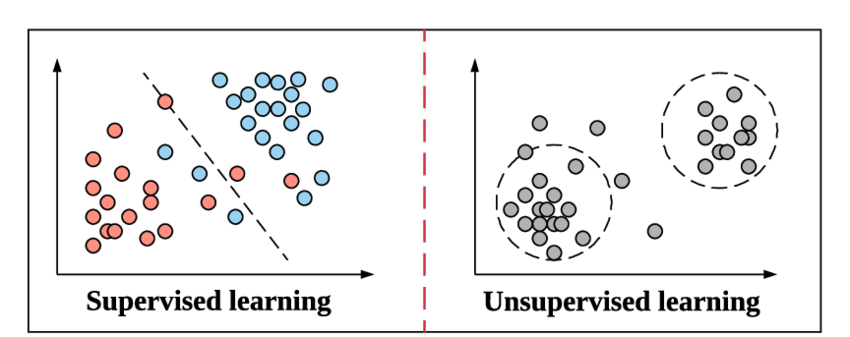
\includegraphics[width=12cm, keepaspectratio]{fig/cap1/Examples-of-Supervised-Learning-Linear-Regression-and-Unsupervised-Learning.png}
	\caption{Diferența dintre modul de funcționare al învățării supervizare și învățării nesupervizate \cite{qian2019orchestrating}}
	\label{fig:sup_and_unsup_learning}
\end{figure}

\subsection*{Învățarea cu întărire}
Învățarea cu întărire este o metodă de învățare prin interacțiuni repetate a unui \textit{agent (software agent)} cu mediul, cu urmărirea atingerii unui anumit scop (\autoref*{fig:reinf_learning}). Interacțiunile se bazează pe acțiunile luate de agent la stimulii mediului, pentru care va primit o recompensă de la acesta în funcție de beneficiul adus îndeplinirii scopului. Recompensele primite au rolul de a îmbunătății capacitatea agentului de a lua cea mai bună decizie din starea în care acesta se afla la momentul acțiunii. Scopul pe termen lung al agentului îl reprezintă maximizarea numărului de recompense primite, astfel încât, după repetate interacțiuni cu mediul, capacitatea acestuia de a lua decizii bune să se îmbunătățească.
\begin{figure}[H]
	\center
	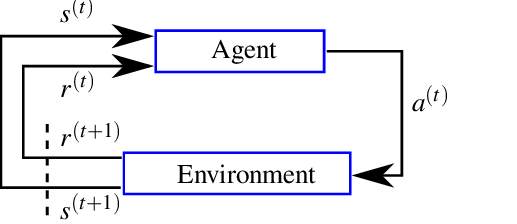
\includegraphics[width=11cm, keepaspectratio]{fig/cap1/The-reinforcement-learning-paradigm-consists-of-an-agent-interacting-with-an.png}
	\caption{Modul de funcționare al învățării cu întărire \cite{fig:reinforcement}}
	\label{fig:reinf_learning}
\end{figure}

\section{Soluții existente}
Apariția unor soluții comerciale \textit{low-cost} non-invazive a facut posibilă înregistrarea și analiza undele cerebrale în afara domeniului medical \cite{online:emotiv}. În principal, aceste dispozitive sunt folosite în activități simple de interfațare a creierului cu calculatorul \textit{(BCI - Brain-Computer Interface)}. Raportul zgomot-semnal util mare și eșantionarea imperfectă reprezentând dezavantajele acestor aparate comparativ cu cele de nivel medical. Acest lucru însă nu a împiedicat apariția a tot mai multor studii care folosesc aceste aparate \cite{consumer-eeg:2018}. Studiile care au influențat abordarea acestei teme prezintă soluții în clasificarea stărilor mentale folosind diverse tehnici ale învățarii automate supervizate.

Lucrarea \cite{eeg:2018} studiază diferite metode de extragere a informației din semnalele EEG, reprezentând trei stări mentale diferite, sub forma unor atribute, pe baza cărora este creat un set de date. Acestui set de date rezultat îi este redusă apoi dimensionalitatea, alegând doar cele mai relevate antribute, folosind diverși algoritmi, precum algoritmi evolutivi \textit{(Evolutionary Algorithm)}, corelația atributelor, \textit{OneR} și altele. Sunt studiați diferiți algoritmi pentru clasificarea datelor pe seturile de date rezultate după aplicarea metodelor de selecție a atributelor. Printre algortmii folosiți se numără Bayes Naiv, SVM, \textit{Random Forest} și altele. Cele mai bune rezultate au fost obținute folosind setul de date rezultat prin aplicarea algoritmului OneR împreună cu clasificatorul Random Forest, acuratețea modelului ajungând la valoarea de $87.16\%$.

Folosind informațiile și metoda de lucru propusă în \cite{eeg:2018}, lucrarea \cite{eeg-cnn:2020} dezvoltă arhitectura unei rețele neuronale convoluționale cu scopul de a clasifica cele trei stări mentale, neutru, concentrat și relaxat. Această lucrare preia setul de date inițial creat de lucrarea \cite{eeg:2018} și extrage din acesta un număr de 256 de atribute pentru a crea o imagine alb-negru de dimensiunea $16\times16$. După antrenarea modelului rețelei convoluționale folosind aceste imagini, acuratețea acestuia de prezicere este de $89.38\%$, un avans comparativ cu lucrarea inițială.  

\section{Structurare pe capitole}
Lucrarea este structurată după cum urmează. \textit{\autoref{ch:2studiu_teoretic}} prezintă bazele teoretice ale rețelelor neuronale de tip \textit{feedforward}, iar mai apoi sunt prezentate rețelele neuronale convoluționale, care folosesc la baza lor concepte provenite de la rețelele neuronale simple. Tot în \autoref{ch:2studiu_teoretic} sunt prezentate și concepte fundamentale referitoare la undele cerebrale, ce sunt acestea, cum funcționează și felul în care pot fi detectate și înregistrate. În \textit{\autoref{ch:3implementare}} este prezentată implementarea soluției propuse, împreună cu detaliile tehnice aferente. Explicarea tehnicilor de extragere și prelucrare a datelor, detalii privind arhitectura rețelei folosite și rezultatele produse de aceasta se regăsesc la finalul acestui capitol. Finalul lucrarii este alcătuit din \textit{\autoref{ch:4concluzii}}, care aduce concluzii legate de tema acestei lucrări.